\appendix
%\chapter{Proof of Theorem 1}\label{appendix1}

\begin{comment}
\chapter{提案手法のアルゴリズム}\label{appendix3}

\section{動作学習のアルゴリズム}

与えられた教示動作を用いて,各観点における確率モデルを更新し,学習を行う.Algorithm \ref{algorithm1}に,提案手法の学習のアルゴリズムを示す.
	\begin{algorithm}[b]
		\caption{ Learning algorithm of the proposed method}
		\label{algorithm1}
		\begin{algorithmic}
			\REQUIRE
				$N$ : the number of training data \\
				$M$ : the number of reference points , 
				$O$ : the number of objects \\
				$D = \{D_{1} , D_{2} , \ldots , D_{N}\}$ : training dataset \\
				$L = \{l_{1} , l_{2} , \ldots , l_{M}\}$ : the candidates of the reference point \\
				$K = \{k_{id} , k_{lt} , k_{gl}\}$ : coordinate systems \\
				$V = <L , K>$ : the candidates of the viewpoints \\
				$μ_{lk}$ : mean of the Probabilistic model of $<l , k>$ \\
				$Q_{lk}$ : mean-square of the Probabilistic model of $<l , k>$ \\
				$σ_{lk}$ : variance of the Probabilistic model of $<l , k>$ \\
				$Transform_{lk}(v)$ : Affine transfomation , 
				$Normalize_{lk}(v)$ : Normalization
		\end{algorithmic}
		\begin{algorithmic}[1]
			\STATE $M \leftarrow 2^{O}$
			
			\FOR{$n=1$ to $N$}
				\STATE $d \leftarrow D_{n}$
				\FOR{$m=1$ to $M$}
					\FOR{all $k ∈K$}
						\STATE $d_{l_{m}k} \leftarrow Normalize_{l_{m}k}(Transform_{l_{m}k}(d))$
						\STATE $μ_{l_{m}k} \leftarrow \frac{n-1}{n}μ_{l_{m}k} + \frac{1}{n}d_{l_{m}k}$
						\STATE $Q_{l_{m}k} \leftarrow \frac{n-1}{n}Q_{l_{m}k} + \frac{1}{n}(d_{l_{m}k})^2$
						\STATE $σ_{l_{m}k} \leftarrow Q_{l_{m}k} - (μ_{l_{m}k})^2$
					\ENDFOR
				\ENDFOR
			\ENDFOR
		\end{algorithmic}
	\end{algorithm}
ここで,$k_{id} , k_{lt} , k_{gl}$は座標系を表し,それぞれ画面に平行,参照点からトラジェクタの初期位置方向,参照点から重心の構成物体方向とする.参照点が複数の物体の重心でない場合,$k_{gl}$は考慮しない.


\section{動作再現のアルゴリズム}

教示動作から学習された各観点における確率モデルを用いて,異なる初期環境での動作再現を行う.Algorithm \ref{algorithm2}に,提案手法の動作再現のアルゴリズムを示す.
	\begin{algorithm}[h]
		\caption{ Reproduction algorithm of the proposed method}
		\label{algorithm2}
		\begin{algorithmic}
			\REQUIRE
				$M$ : the number of reference points \\ 
				$L = \{l_{1} , l_{2} , \ldots , l_{M}\}$ : the candidates of the reference point \\
				$K = \{k_{id} , k_{lt} , k_{gl}\}$ : coordinate systems \\
				$V = <L , K>$ : learned models of the viewpoints \\
				$μ_{lk}$ : mean of the Probabilistic model of $<l , k>$ \\
				$Q_{lk}$ : mean-square of the Probabilistic model of $<l , k>$ \\
				$σ_{lk}$ : variance of the Probabilistic model of $<l , k>$ \\
				$Transform_{lk}(v)$ : Affine transfomation , 
				$Normalize_{lk}(v)$ : Normalization \\
				$Position(l)$ : Position of the reference point $l$
		\end{algorithmic}
		\begin{algorithmic}[1]
			\STATE $<l_{max} , k_{max}> \leftarrow <l_{1} , k_{1}>$
			\FOR{all $<l , k>∈V$}
				\IF{$σ_{lk} < σ_{l_{max}k_{max}}$}
					\STATE $<l_{max} , k_{max}> \leftarrow <l , k>$
				\ENDIF
			\ENDFOR
			\STATE $d \leftarrow Transform^{-1}(Normalize^{-1}(μ_{l_{max}k_{max}}))$
			\STATE $d \leftarrow d + Position(l_{max})$
		\end{algorithmic}
	\end{algorithm}


\section{動作識別のアルゴリズム}

モデルが学習された各動作から例示動作の生起確率を計算することで,例示動作が既学習動作のうちいずれであるか識別を行う.Algorithm \ref{algorithm3}に,提案手法の動作識別のアルゴリズムを示す.
	\begin{algorithm}[h]
		\caption{ Identification algorithm of the proposed method}
		\label{algorithm3}
		\begin{algorithmic}
			\REQUIRE
				$x_{input}$ : the destination of the exemplified task \\ 
				$M$ : the number of reference points , 
				$S$ : the number of learned tasks \\
				$L = \{l_{1} , l_{2} , \ldots , l_{M}\}$ : the candidates of the reference point \\
				$K = \{k_{id} , k_{lt} , k_{gl}\}$ : coordinate systems \\
				$T = \{t_{1} , t_{2} , \ldots t_{S}\}$ : learned tasks \\
				$V_{t} = <L_{t} , K_{t}>$ : learned models of the viewpoints in the task $t$\\
				$μ_{lk}$ : mean of the Probabilistic model of $<l , k>$ \\
				$Q_{lk}$ : mean-square of the Probabilistic model of $<l , k>$ \\
				$σ_{lk}$ : variance of the Probabilistic model of $<l , k>$ \\
				$Transform_{lk}(v)$ : Affine transfomation , 
				$Normalize_{lk}(v)$ : Normalization \\
				$Probability(<i , k> , x)$ : Probability that $x$ is generated from $<l , k>$
		\end{algorithmic}
		\begin{algorithmic}[1]
			\STATE $t_{max} \leftarrow t_{1}$
			\STATE $<l_{max} , k_{max}> \leftarrow <l_[1] , k_[1]>$
			
			\FOR{all $t∈T$}
				\STATE $<l_{max}^{t} , k_{max}^{t}> \leftarrow <l_{1}^{t} , k_{1}^{t}>$
				\FOR{all $<l^{t} , k^{t}>∈V_{t}$}
					\IF{$σ_{l^{t}k^{t}} < σ_{l_{max}^{t}k_{max}^{t}}$}
						\STATE $<l_{max}^{t} , k_{max}^{t}> \leftarrow <l^{t} , k^{t}>$
					\ENDIF
				\ENDFOR
				\IF{$Probability(<l_{max}^{t} , k_{max}^{t}> , v_{input}) > Probability(<l_{max} , k_{max}> , v_{input})$}
					\STATE $<l_{max} , k_{max}> \leftarrow <l_{max}^{t} , k_{max}^{t}>$
					\STATE $t_{max} \leftarrow t$
				\ENDIF
			\ENDFOR
		\end{algorithmic}
	\end{algorithm}

\clearpage
\end{comment}

\chapter{動作再現実験における実験結果}\label{appendix1}

動作の再現実験における,教示誤差と再現誤差の関係を図\ref{figure:errors}に示す.
ここで,横軸は教示誤差の分散,縦軸は再現誤差の標準偏差を表す.
各教示誤差において,教示動作からの学習,再現を行った際の再現誤差を50回ずつ実験を行った.適切な観点が選択されている場合,教示誤差と再現誤差の分散が等しくなることが期待される.即ち各グラフにおいて教示誤差$t$,再現誤差$r$に関して,
\[
	r = \sqrt{t}
\]
という関係が満たされていることが期待される.
\ref{figure:errors}において,付録\ref{appendix2}で述べる成否の判別境界を曲線で示した.
実際のグラフ中には,境界内で無理関数に従うように見える結果と,境界外で相関が見られ難い結果が存在している.
%%%%%%%%%%%%%%%%%%%%%%%%%%%%%%%%%%%%%%%%%%%%%%%%%%%%%%%%%%%%%%%%%%%%%%%%%%%%%%%%%%%%%%%%%%%%%%%%%%%%%%%
\begin{figure}[h]
	\centering
	\begin{minipage}[t]{.49\textwidth}
		\centering
		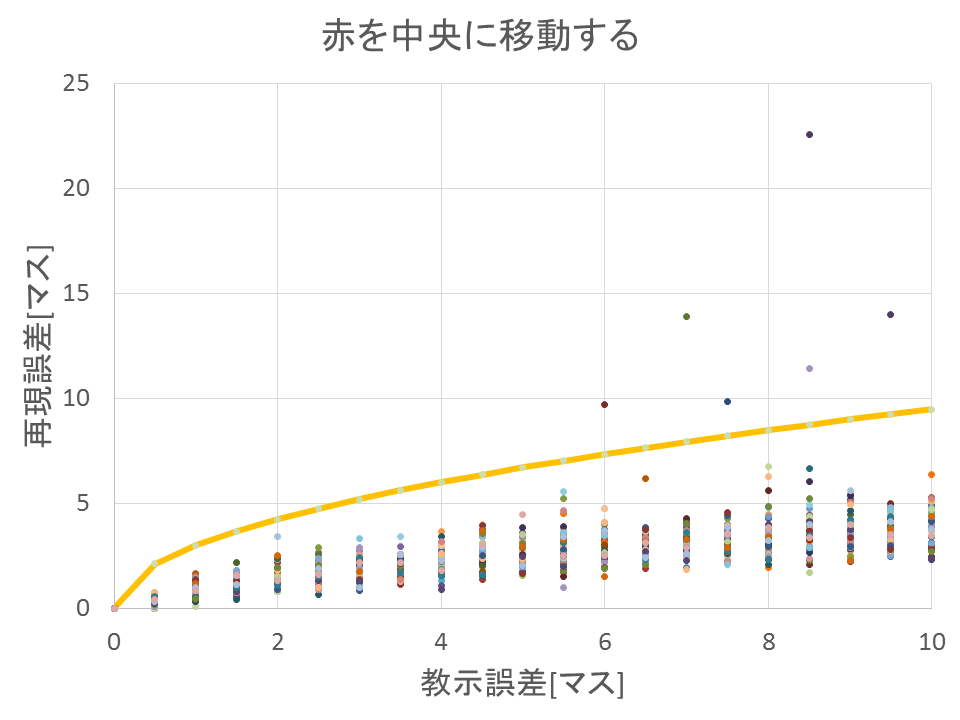
\includegraphics[width=7.5cm]{スライド2.PNG} \\ %TeXの基本として, \\ で緊急改行ができる.(今回の場合や行列などを除き,あまり使わない)
		\subcaption{$T_{1}$:赤を中央に移動する}
		\label{subfig:unit_a}    
	\end{minipage}
	\begin{minipage}[t]{.49\textwidth}
		\centering
		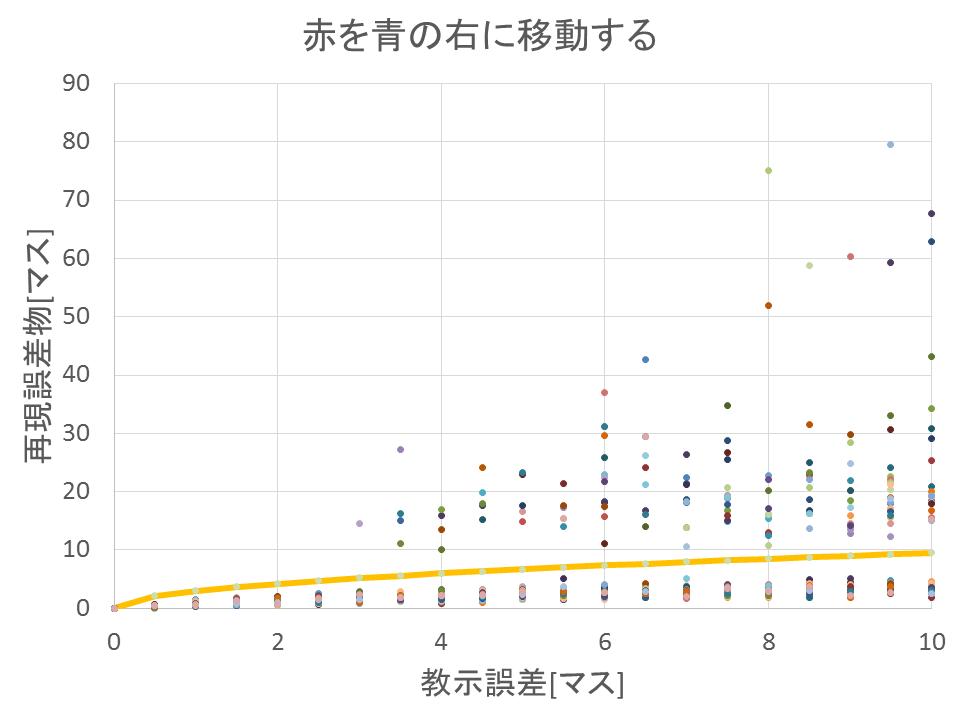
\includegraphics[width=7.5cm]{スライド3.PNG} \\ %TeXの基本として, \\ で緊急改行ができる.(今回の場合や行列などを除き,あまり使わない)
		\subcaption{$T_{2}$:赤を青の右に動かす}
		\label{subfig:unit_b}
	\end{minipage}
	\begin{minipage}[t]{.49\textwidth}
		\centering
		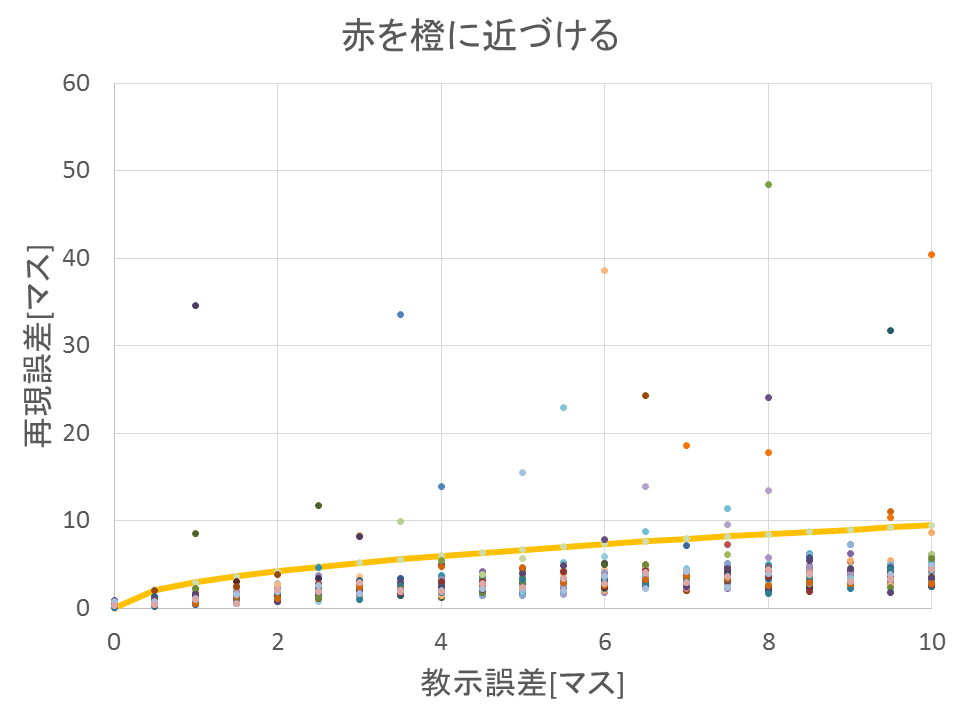
\includegraphics[width=7.5cm]{スライド4.PNG} \\ %TeXの基本として, \\ で緊急改行ができる.(今回の場合や行列などを除き,あまり使わない)
		\subcaption{$T_{3}$:赤を橙に近づける}
		\label{subfig:unit_c}
	\end{minipage}
	\begin{minipage}[t]{.49\textwidth}
		\centering
		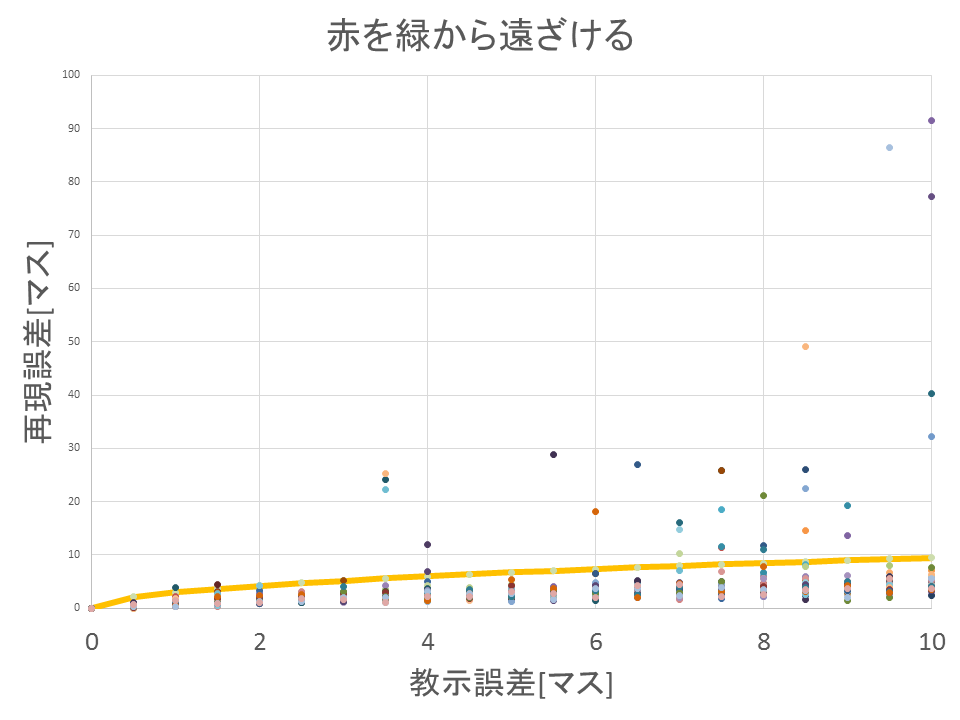
\includegraphics[width=7.5cm]{スライド5.PNG} \\ %TeXの基本として, \\ で緊急改行ができる.(今回の場合や行列などを除き,あまり使わない)
		\subcaption{$T_{4}$:赤を緑から遠ざける}
		\label{subfig:unit_d}
	\end{minipage}
	\begin{minipage}[t]{.49\textwidth}
		\centering
		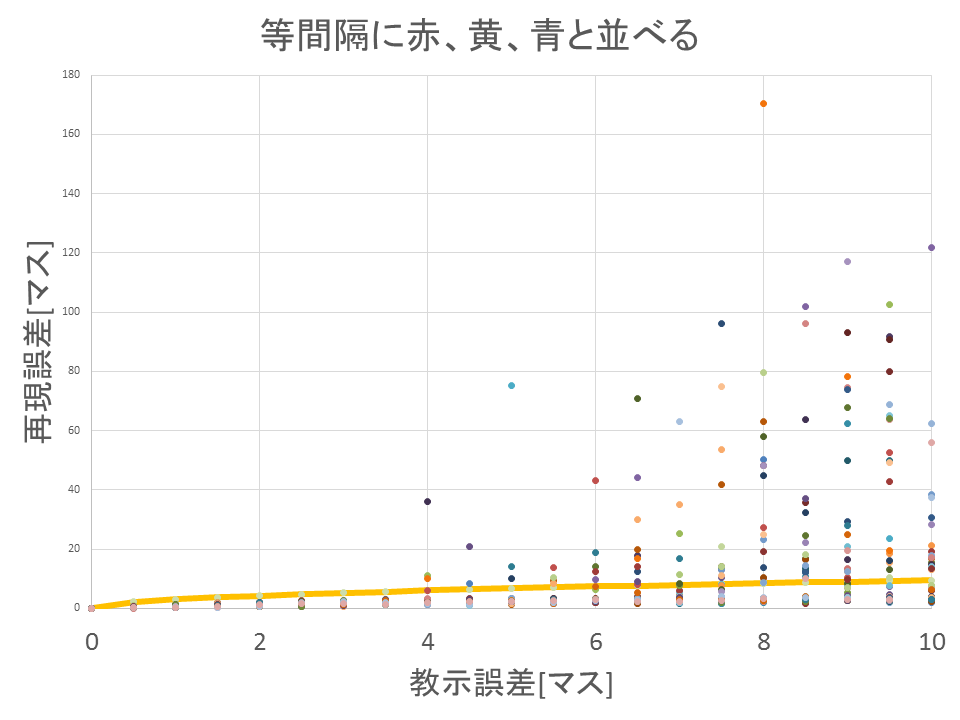
\includegraphics[width=7.5cm]{スライド6.PNG} \\ %TeXの基本として, \\ で緊急改行ができる.(今回の場合や行列などを除き,あまり使わない)
		\subcaption{$T_{5}$:等間隔に赤黄青と並べる}
		\label{subfig:unit_d}
	\end{minipage}
	\begin{minipage}[t]{.49\textwidth}
		\centering
		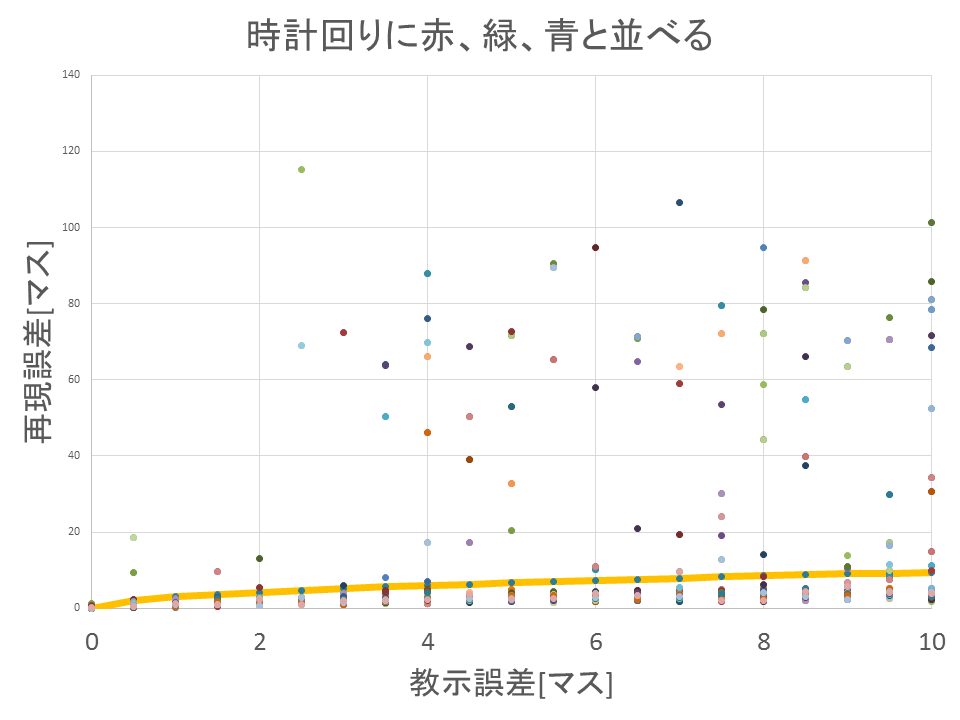
\includegraphics[width=7.5cm]{スライド7.PNG} \\ %TeXの基本として, \\ で緊急改行ができる.(今回の場合や行列などを除き,あまり使わない)
		\subcaption{$T_{6}$:時計回りに赤緑青と並べる}
		\label{subfig:unit_d}
	\end{minipage}
	\caption{教示誤差と再現誤差}
	\label{figure:errors}
\end{figure}
%%%%%%%%%%%%%%%%%%%%%%%%%%%%%%%%%%%%%%%%%%%%%%%%%%%%%%%%%%%%%%%%%%%%%%%%%%%%%%%%%%%%%%%%%%%%%%%%%%%%%%%

\begin{comment}
%%%%%%%%%%%%%%%%%%%%%%%%%%%%%%%%%%%%%%%%%%%%%%%%%%%%%%%%%%%%%%%%%%%%%%%%%%%%%%%%%%%%%%%%%%%%%%%%%%%%%%%
	\begin{figure}
%中央ぞろえ
		\begin{center}
			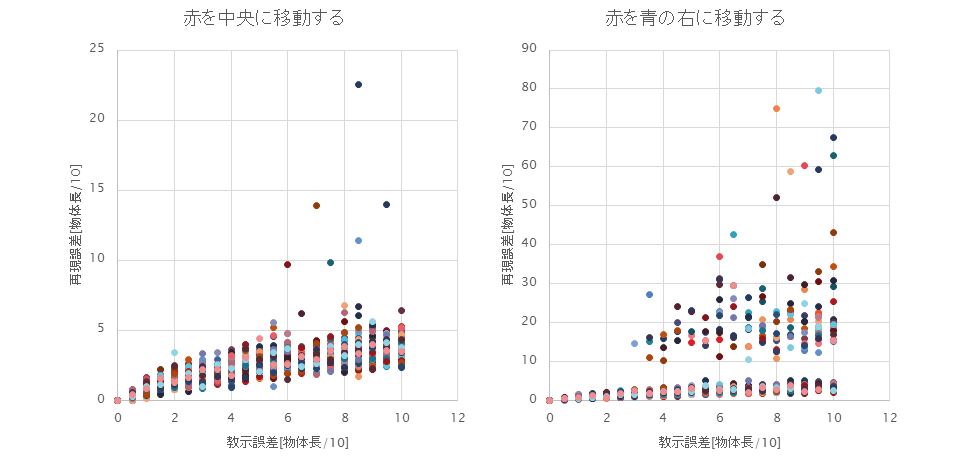
\includegraphics[width=15.5cm]{chart6.png} \\ %eXの基本として, \\ で緊急改行ができる.(今回の場合や行列などを除き,あまり使わない)
			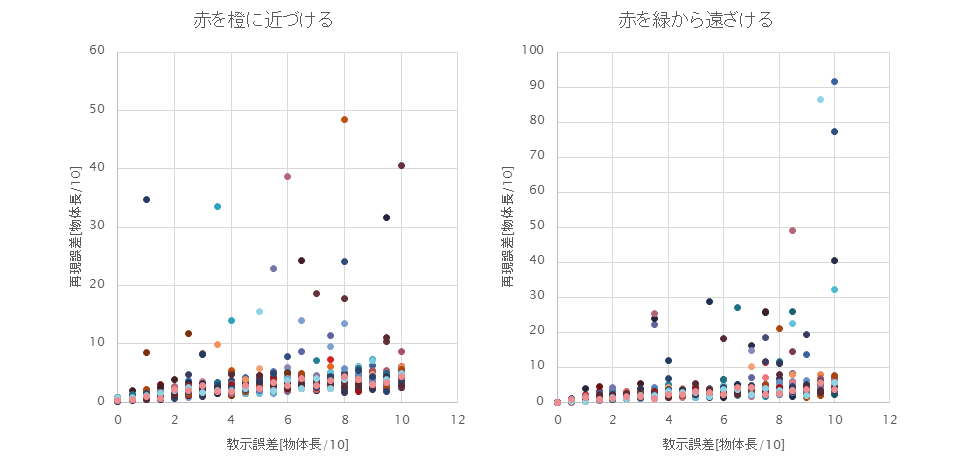
\includegraphics[width=15.5cm]{chart7.png} \\ %eXの基本として, \\ で緊急改行ができる.(今回の場合や行列などを除き,あまり使わない)
			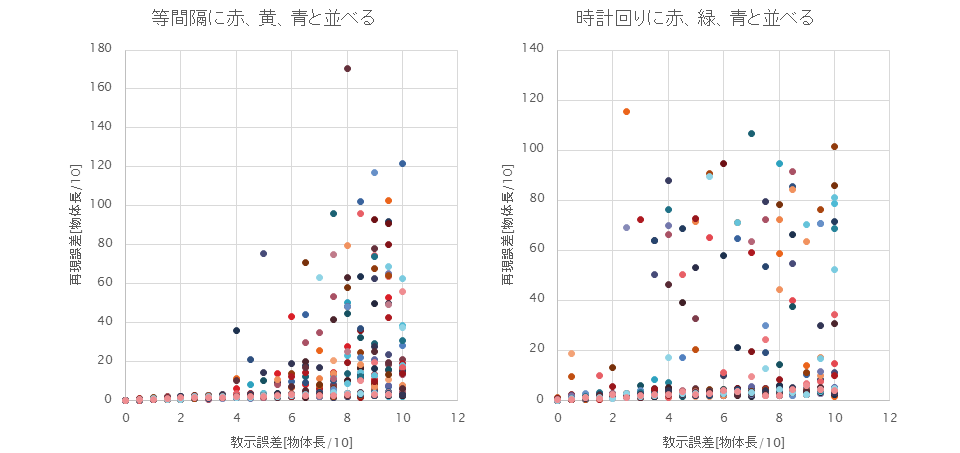
\includegraphics[width=15.5cm]{chart8.png} \\ %eXの基本として, \\ で緊急改行ができる.(今回の場合や行列などを除き,あまり使わない)
			\caption{教示誤差と再現誤差}
			\label{figure:errors}
		\end{center}
	\end{figure}
%%%%%%%%%%%%%%%%%%%%%%%%%%%%%%%%%%%%%%%%%%%%%%%%%%%%%%%%%%%%%%%%%%%%%%%%%%%%%%%%%%%%%%%%%%%%%%%%%%%%%%%
\end{comment}

\chapter{動作再現における観点推定の成否の判定}\label{appendix2}

教示動作から学習したモデルを用いた動作再現を行う際,教示動作自体に誤差が含まれている場合,一つ抜き法によるテスト時に使用するデータも教示動作の一つであるために必然的に誤差が生じる.そのため一つ抜き法により計算された再現誤差が教示誤差に依るものなのか誤学習に依るものなのかを区別する基準が必要である.ここでは正規分布から生成された誤差を含む教示動作から適切に学習された場合に再現誤差も正規分布に従うことを示し,正規分布の性質から観点推定の成否の基準値を設定する.
まず,適切な観点(原点となる参照点と座標系)からの$N$回分の各教示動作における目標位置$Θ=\{θ_{1} , θ_{2} , \ldots , θ_{N}\}$に対し,$Θ$を用いた一つ抜き法による評価値を次のように求める.
	\begin{equation}
		\label{CrossVaridation}
		Cr(Θ) = \frac{1}{N} \sum_{n=1}^{N} F(θ_{n} | Θ \backslash θ_{n})
	\end{equation}
ここで\ref{CrossVaridation}式の右辺$F(θ_{n} | Θ \backslash θ_{n})$は,$θ_{n}$を除く$Θ$を用いて学習し再現を行った結果の目標位置と$θ_{n}$の誤差を表す.動作再現は選択された観点に割り当てられた正規分布の平均を出力するので,
	\begin{equation}
		\label{F}
		F(θ_{n} | Θ \backslash θ_{n}) = |θ_{n} - mean(Θ \backslash θ_{n})| = |\frac{N}{N-1}(θ_{n} - mean(Θ))|
	\end{equation}
である.ただし$mean(A)$はAの平均とする.\ref{F}式を\ref{CrossVaridation}に代入すると
	\begin{equation}
		\label{Cr2}
		Cr(Θ) = \frac{1}{N} \sum_{n=1}^{N}  |\frac{N}{N-1}(θ_{n} - mean(Θ))|
		 = \frac{N}{N-1}\frac{1}{N}  \sum_{n=1}^{N}  |(θ_{n} - mean(Θ))| 
	\end{equation}
と整理できる.ここで\ref{Cr2}式の右辺$|(θ_{n} - mean(Θ))|$は$θ_{n}$の持つガウス誤差と等しいので,
	\begin{equation}
		\label{Cr3}
		mean(Cr(Θ)) = \frac{N}{N-1} * mean(\frac{1}{N}  \sum_{n=1}^{N}  |(θ_{n} - mean(Θ))| )
		 = \frac{N}{N-1} * mean(|G_{error}|)
	\end{equation}
となる.$2\int_{0}^{\infty}G_{error}(v)dv = \sqrt{\frac{2}{\pi}}σ$であることから,$Cr(Θ)$の平均は
	\begin{equation}
		\label{Cr4}
		mean(Cr(Θ)) = \frac{N}{N-1}\sqrt{\frac{2}{\pi}}σ
	\end{equation}
と求められる.ただし$σ$はガウス誤差の分散である.同様に,
	\begin{equation}
		\label{Cr^2_1}
		mean(Cr(Θ)^2) = \left(\frac{N}{N-1}\right)^2 * mean(|G_{error}|^2) 
		= 2\int_{0}^{\infty}\frac{x^2}{\sqrt{2\pi}σ}e^{-\frac{x^2}{2σ^2}}dx
	\end{equation}
であり,これを計算することで,
	\begin{equation}
		\label{Cr^2_2}
		mean(Cr(Θ)^2) = \left(\frac{N}{N-1}\right)^2 σ^2
	\end{equation}
が得られる.\ref{Cr4}式と\ref{Cr^2_2}式から,$Cr(Θ)$の標準偏差は,
	\begin{equation}
		\sqrt{V(Cr(Θ))} = \sqrt{mean(Cr(Θ)^2) - \left(mean(Cr(Θ))\right)^2} = \frac{N}{N-1}\sqrt{\frac{\pi-2}{\pi}}σ
	\end{equation}
と求められる.平均$m$,分散$σ$の正規分布に従うデータ$θ$に対して$|θ-m|>3σ$となる確率は99.73\%となることが知られている.このような$θ$は,適切な観点でない異なる分布から生起されたとし,観点の推定自体を誤っていると考えることで,観点推定の成否を判定し評価することができる.今回の実験において$θ>0$であるため,基準値$θ_{border}$を,
	\begin{equation}
		θ_{border} = mean(Cr(Θ))+3\sqrt{V(Cr(Θ))}≒2.8959σ
	\end{equation}
と定め,これ以上の再現誤差が生じた結果について観点推定失敗と定めた.



%\chapter{Proof of Theorem 2}\label{appendix2}
%\chapter{定理2の証明}\label{appendix2}
